\documentclass[border=4pt]{standalone}
\usepackage{fontspec}
\usepackage{amsmath}
\usepackage{unicode-math}
\setmainfont{Latin Modern Roman}
\setmathfont{Latin Modern Math}
\usepackage{pgfplots}
\usepackage{pgfplotstable}
\pgfplotsset{compat=1.18}
\usepackage{tkz-euclide}
\usetikzlibrary{arrows.meta,calc,angles,quotes,patterns,3d,backgrounds}
\definecolor{ink}{HTML}{123428}
\definecolor{asy}{HTML}{475569}
\definecolor{mint}{HTML}{86e0bd}
\tikzset{asym/.style={asy, line width=0.9pt, dash pattern=on 5pt off 3.5pt},
         guide/.style={gray!70, line width=0.6pt, densely dotted},
         dot/.style={circle, inner sep=0pt, minimum size=5pt, draw=white, line width=0.5pt},
         odot/.style={circle, inner sep=0pt, minimum size=5.5pt, fill=white, line width=1pt},
         lab/.style={font=\footnotesize, inner sep=1.5pt, text=ink}}
\begin{document}
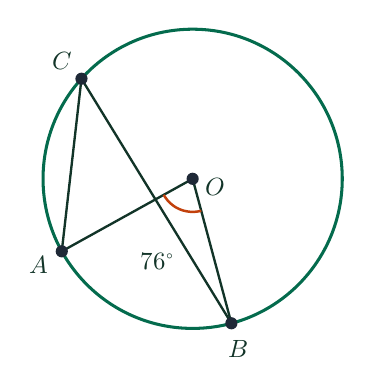
\begin{tikzpicture}
\draw[color={rgb,255:red,4;green,107;blue,77}, line width=1.1pt] (0,0) circle (1.900);
\draw[ink, line width=0.85pt] (-1.412,1.271) -- (-1.662,-0.921);
\draw[ink, line width=0.85pt] (-1.412,1.271) -- (0.492,-1.835);
\draw[ink, line width=0.85pt] (0.000,0.000) -- (-1.662,-0.921);
\draw[ink, line width=0.85pt] (0.000,0.000) -- (0.492,-1.835);
\draw[color={rgb,255:red,194;green,65;blue,12}, line width=0.9pt] (-0.367,-0.204) -- (-0.353,-0.228) -- (-0.337,-0.250) -- (-0.320,-0.272) -- (-0.301,-0.293) -- (-0.281,-0.312) -- (-0.260,-0.330) -- (-0.237,-0.347) -- (-0.214,-0.362) -- (-0.189,-0.375) -- (-0.164,-0.387) -- (-0.138,-0.397) -- (-0.112,-0.405) -- (-0.084,-0.411) -- (-0.057,-0.416) -- (-0.029,-0.419) -- (-0.001,-0.420) -- (0.026,-0.419) -- (0.054,-0.417) -- (0.082,-0.412) -- (0.109,-0.406);
\node[font=\small, text=ink, inner sep=0.5pt, fill=white] at (-0.445,-1.049) {$76^\circ$};
\fill[color={rgb,255:red,31;green,41;blue,55}] (-1.662,-0.921) circle (2.2pt);
\fill[color={rgb,255:red,31;green,41;blue,55}] (0.492,-1.835) circle (2.2pt);
\fill[color={rgb,255:red,31;green,41;blue,55}] (-1.412,1.271) circle (2.2pt);
\fill[color={rgb,255:red,31;green,41;blue,55}] (0.000,0.000) circle (2.2pt);
\node[font=\small, text=ink, inner sep=0.5pt] at (-1.959,-1.086) {$A$};
\node[font=\small, text=ink, inner sep=0.5pt] at (0.580,-2.164) {$B$};
\node[font=\small, text=ink, inner sep=0.5pt] at (-1.665,1.499) {$C$};
\node[font=\small, text=ink, inner sep=0.5pt] at (0.282,-0.103) {$O$};
\end{tikzpicture}
\end{document}
